\begin{KR}{Zusammenhänge:}\\
    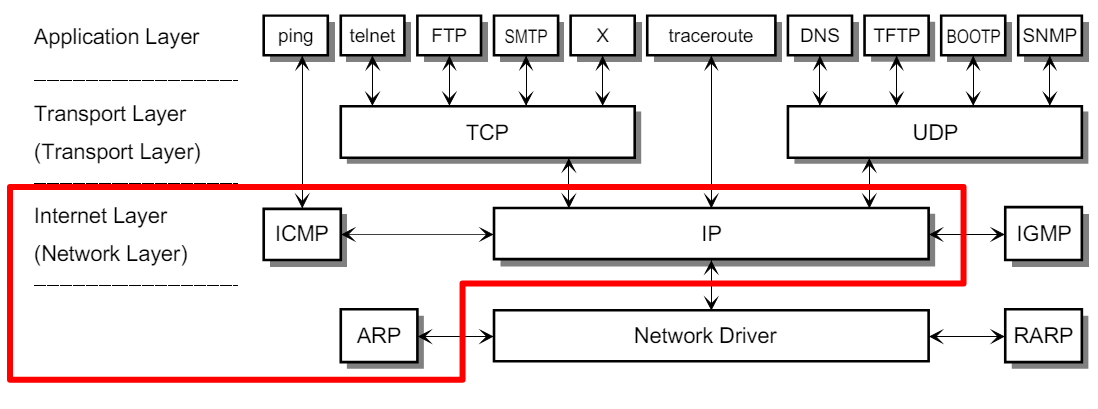
\includegraphics[width=1\linewidth]{images/orientierung_network_layer.png}
    \end{KR}

\section{Transport Layer}
\paragraph{Schicht 4: Transportschicht}

\begin{definition}{Kapselung} Protocol-Feld unterscheidet UDP und TCP Daten
    
    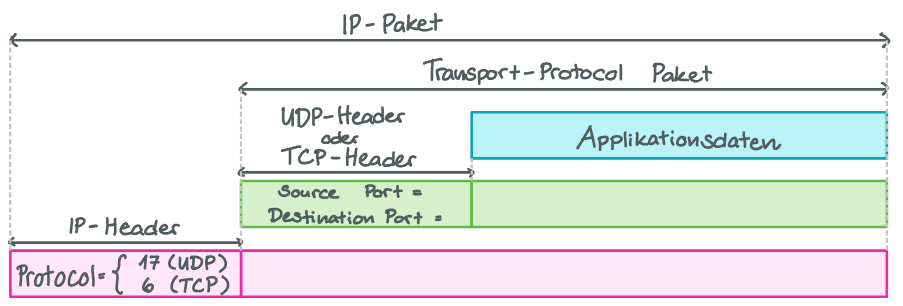
\includegraphics[width=1\linewidth, height=0.3\linewidth]{images/tcp_udp_header.png}
\end{definition}

\begin{concept}{Adressierung}
    {\small Client adressiert Server-Appl. mit Destination Port Nr.}
    \begin{itemize}
        \item sonst weiss TCP/UDP-Modul im Empfänger nicht, welche Applikation gemeint ist
        \item für Source Port Nummer verwendet Client (meist) zufällige Port Nummer >1'023 (vom Betriebssystem vergeben)
    \end{itemize}
\end{concept}

\paragraph{UDP - User Datagram Protocol}

\begin{definition}{UDP}
    Multi-/Demultiplexen: anhand Portnummern Daten den richtigen Applikationen zuweisen
    $\Rightarrow$ Verbindungslos und unzuverlässig\\
    {\small Vorteile: simpel, wenig Overhead, kein Verbindungsaufbau (schnell)}
\end{definition}

\begin{concept}{UDP-Header}
    \begin{itemize}
        \item \textcolor{darkfrog}{Source/Destination Port} Sendende/Empfänger Applikation
        \item \textcolor{blue}{Message Length} Länge des Datagramms
        \item \textcolor{darkpurple}{Checksum} Prüfsumme über einen Pseudo-Header, UDP-Header und Daten (kann Null sein)
    \end{itemize}
        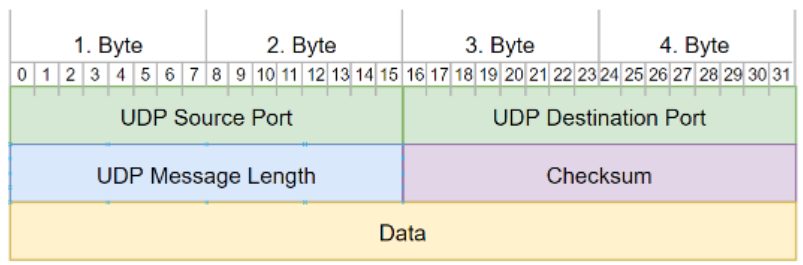
\includegraphics[width=0.8\linewidth, height=0.25\linewidth]{images/udp.png}
\end{concept}

\begin{remark}
    Pseudo-Header: IP Source- und Destination Address, Protocol Feld, Länge des Datagramms
            $\rightarrow$ fehlgeleitete Datagramme können erkannt werden
\end{remark}

\begin{formula}{Port-Nummern}
    \begin{itemize}
        \item \textcolor{darkfrog}{System Ports (Well-Known)} Fix, für bekannte Appl. reserviert
        \item \textcolor{blue}{User Ports (Registered)} Reserviertert für herstellerspez. Appl.
        \item \textcolor{darkcorn}{Dynamic/Private Ports} Frei verfügbare Ports
    \end{itemize}
        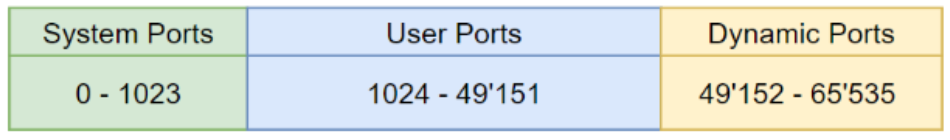
\includegraphics[width=0.7\linewidth, height=0.1\linewidth]{images/portnummern.png}
\end{formula}

\paragraph{TCP - Transmission Control Protocol}

\begin{definition}{TCP Eigenschaften} 
    Verbindungsorientierte Übertragung, zuverlässiger Verbindungsaufbau, hohe Zuverlässigkeit, Vollduplexübertragung, Stream-Schnittstelle, Graceful Termination, Punkt-zu-Punkt Kommunikation
\end{definition}

\begin{concept}{TCP-Header Format}
    \begin{itemize}
        \item \textcolor{darkcorn}{Sequence-Nr.} {\small Sicherstellung Reihenfolge, Erkennung lost Data}
        \item \textcolor{darkcorn}{Acknowledgement-Nr.} {\small n+1: Daten bis \& mit n korrekt/vollständig}
        \item \textcolor{darkpurple}{Data Offset} Gibt an wo Daten beginnen / enden
        \item \textcolor{darkpurple}{ECN-Flags} Explicit Congestion Notification
        {\small
        \begin{itemize}
            \item Bit 8: CWR (Congestion Window Reduced)
            \item Bit 9: ECE (ECN-Echo)
        \end{itemize}}
        \item \textcolor{darkpurple}{Control Bits} Verbindungsauf- und -abbau (Bits 10-15)
        \item \textcolor{blue}{Window} Verfügbare Puffergrösse 
        \item \textcolor{darkpurple}{Urgent Pointer} URG = 1 → Position der wichtigen Daten
        \item \textcolor{darkpurple}{Options} häufigste Verwendung: MSS (Maximum Segment Size)
    \end{itemize}
    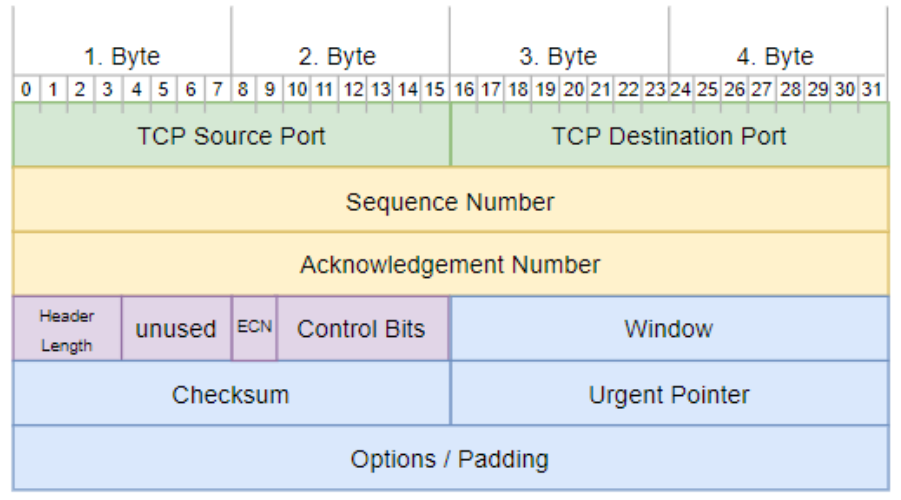
\includegraphics[width=0.8\linewidth, height=0.36\linewidth]{images/tcpheader.png}
\end{concept}

\begin{remark} Control Bits:
    URG: Urgent Pointer,
        ACK: Acknowledgement Number (Bestätigung empfangener Daten, Erkennung verlorener Daten),\\
        PSH: Push (sofort ohne buffern weiterleiten),
        RST: Reset (Verbindung zurücksetzen oder geschlossenen Port signalisieren),
        SYN: Verbindungsaufbau,
        FIN: Verbindungsabbau
\end{remark}

\begin{comment}
\begin{concept}{Verbindungsorientierte Kommunikation}\\
    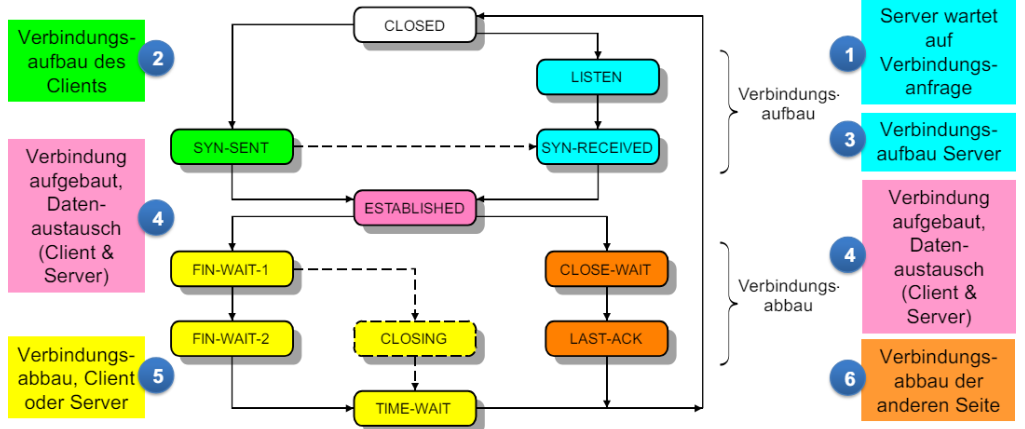
\includegraphics[width=1\linewidth]{images/zustandsdiagramm_tcp.png}
\end{concept}

\end{comment}

\begin{formula}{Herausforderungen} zur Zuverlässigkeit zwischen Ethernet/TCP:\\
    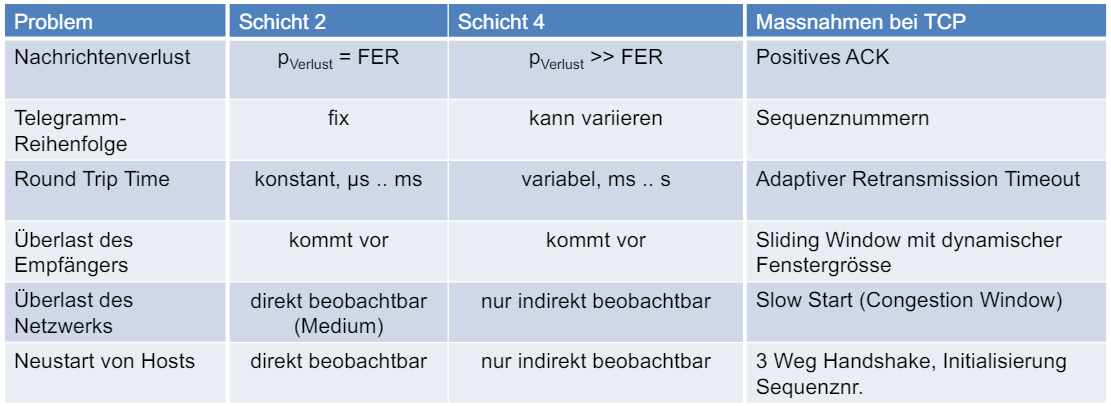
\includegraphics[width=1\linewidth]{images/vergleich_layer_2_4.png}
\end{formula}

\paragraph*{Timed Delays}

\begin{formula}{Round Trip Time (RTT)}
    dynamische Anpassung der Wartezeit 
    \begin{itemize}
        \item  $\textcolor{blue}{SRTT_n} = (1 - \alpha) \cdot \textcolor{blue}{SRTT_{n-1}} + \alpha \cdot \textcolor{green}{RTT_n}$
        \item $\textcolor{Goldenrod}{RTTVAR_n} = (1 - \beta) \cdot \textcolor{Goldenrod}{RTTVAR_{n-1}} + \beta \cdot \textcolor{blue}{SRTT_n} - \textcolor{green}{RTT_n}$
        \item $RTO_n = \textcolor{blue}{SRTT_n} + 4 \cdot \textcolor{Goldenrod}{RTTVAR_n}$
    \end{itemize}
    {\small $\alpha = 0.125, \beta = 0.25$ sind Standardwerte}
\end{formula}

\begin{minipage}{0.7\linewidth}
\begin{formula}{Bandwidth Delay Product (TCP-Puffergrössen)}\\
        Wahl der Grösse von Sende- und Empfangspuffer, um Verbindung nicht auszubremsen\\
        $BDP (bits) = RTT (sec) \cdot Bandbreite (bps)$
\end{formula}
\end{minipage}
\begin{minipage}{0.29\linewidth}
    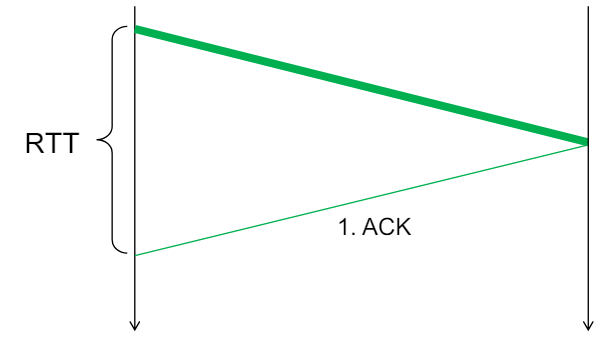
\includegraphics[width=1\linewidth]{images/bdp_rtt.png}    
\end{minipage}


\begin{KR}{Verbindungsaufbau und Verbindungsabbau}\\
\begin{minipage}{0.49\linewidth}
        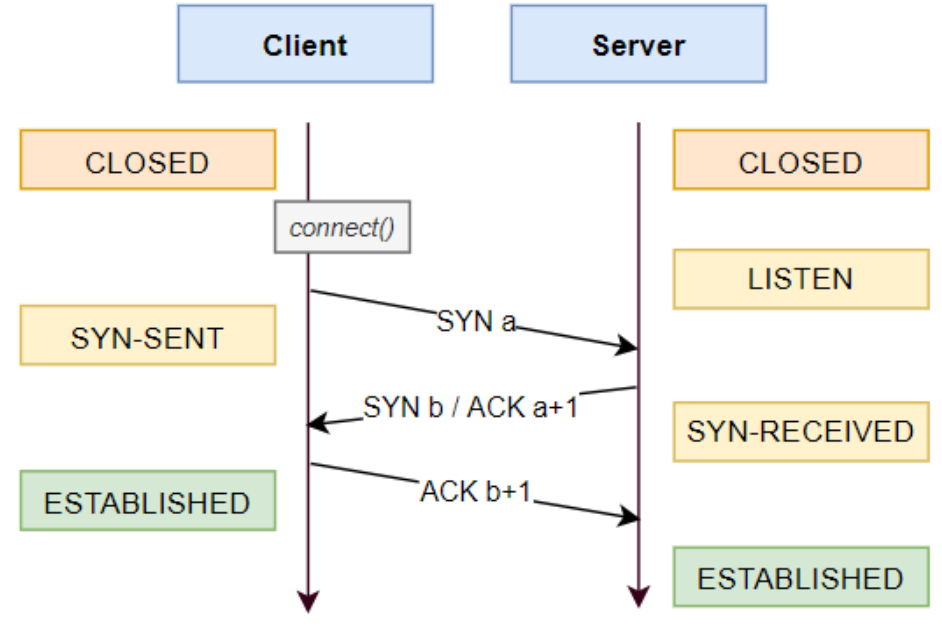
\includegraphics[width=1\linewidth]{images/verbindungsaufbau.png}
\end{minipage}
\begin{minipage}{0.5\linewidth}
        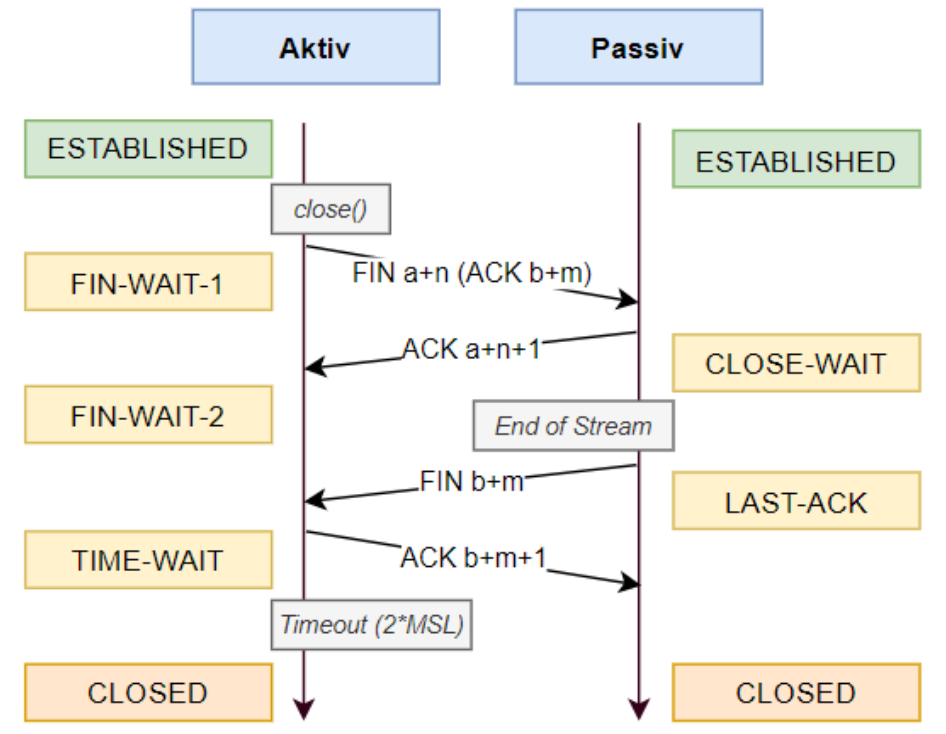
\includegraphics[width=1\linewidth]{images/Verbindungsabbau.png}
\end{minipage}

{\small ACK nr. mit Anzahl Bits der empfangenen Daten aktualisieren!!}
\end{KR}

\paragraph*{Vollständiges Beispiel}

\begin{example}
    Verbindungsaufbau:
    \begin{itemize}
        \item Server: (LISTEN) auf bestimmten Port Nummer
        \item Client: sendet Segment mit SYN=1 und zufälliger init. Sequenznummer a (ACK=0, weil ACK nr. ungültig)
        \item Server bestätigt Sequenznummer mit ACK nr. a+1 und ACK=1, wählt zufällige initiale Sequenznummer b, setzt SYN=1
        \item Client bestätigt b mit ACK nr. b+1 
        \begin{itemize}
            \item Erstes Byte vom Client zum Server hat Sequenznummer a+1
            \item Erstes Byte vom Server zum Client hat Sequenznummer b+1
        \end{itemize}
    \end{itemize}
    \centering
        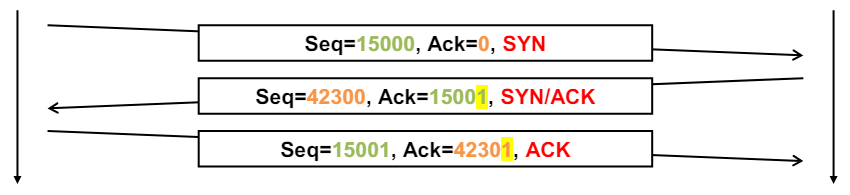
\includegraphics[width=0.8\linewidth]{images/example_verbindungsaufbau_tcp.png}
\end{example}

\begin{example}
    Datenaustausch: TCP-Nachrichten werden bi-direktional ausgetauscht\\
    \centering
    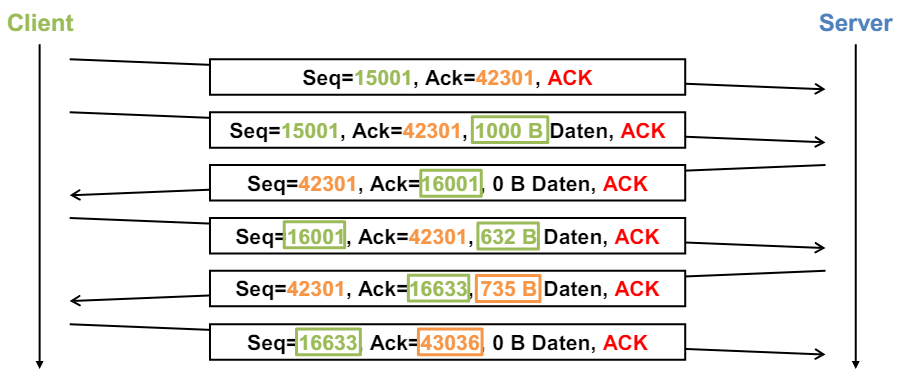
\includegraphics[width=0.8\linewidth]{images/tcp_datenaustausch_ex.png}
\end{example}

\begin{example}
    Beide Seiten können den Verbindungsabbau einleiten
    \begin{itemize}
        \item Ist eine Richtung geschlossen (FIN, ACK), so können in die andere Richtung immer noch Daten gesendet werden (Half-Closed)
        \begin{itemize}
            \item In Richtung der "geschlossenen" Verbindung wird nicht mehr kommuniziert (Acknowledge number mismatch)
        \end{itemize}
        \item Falls die zweite Seite die Verbindung auch schliesst, können die 3. und die 4. Nachricht zusammengefasst werden → FIN/ACK
    \end{itemize}
    \centering
        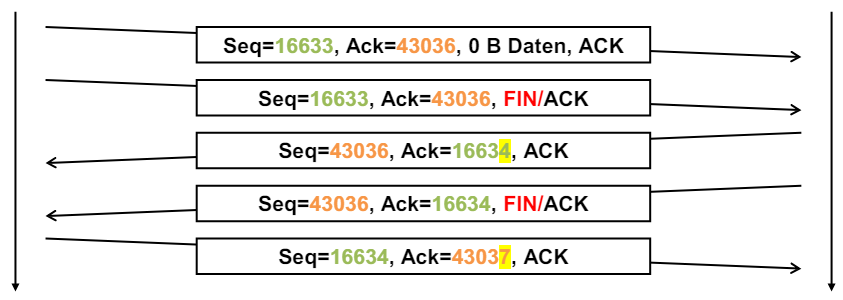
\includegraphics[width=0.8\linewidth]{images/tcp_verbindungsabbau_ex.png}
\end{example}


\begin{remark}
    Mehrere Clients wollen gleichzeitig auf denselben Server zugreifen?\\
    Verbindungsanfragen (SYN) kommen nacheinander zum Server. 1. SYN $\rightarrow$ Verbindungsaufbau zum entsprechenden Client. 
    Weiteren Anfragen werden gequeued. Nach Schliessen der 1. Verbindung wird nächste Anfrage der Queue entnommen/behandelt, usw.
\end{remark}




\paragraph*{Fluss-Steuerung und Congestion Control}



\begin{concept}{Fluss-Steuerung} aus Perspektive Sender\\
    Stop-and-Wait: wartet auf Bestätigung bevor er weiter sendet\\
    Sliding Window: sendet mehrere Frames bevor er auf Bestätigung wartet
\end{concept}

\begin{concept}{Congestion Control - Slow Start}\\
    \begin{minipage}{0.6\linewidth}
        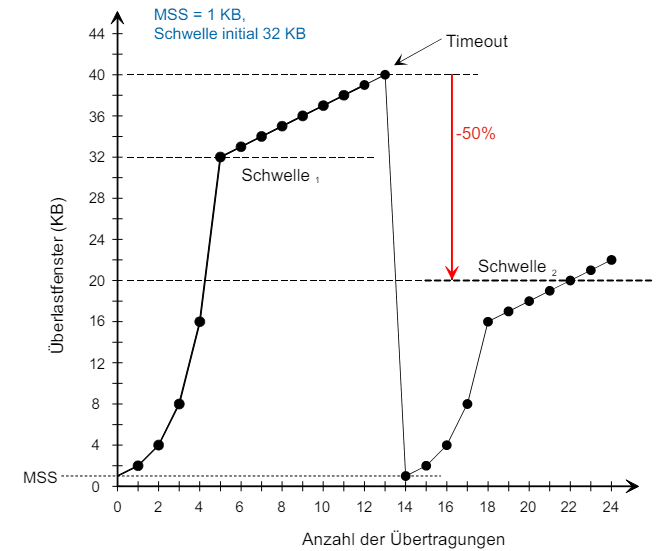
\includegraphics[width=1\linewidth]{images/congestion_control.png}
    \end{minipage}
    \begin{minipage}{0.39\linewidth}
        {\small
        Slow Start: herantasten wie gross die einzelnen Frames sein können.

        \vspace{1mm}

        \textcolor{pink}{Wichtig:} Sender kombiniert Congestion Window mit\\ Informationen zur Flow\\ Control vom Empfänger\\ $\rightarrow$ schickt unbestätigte \\Daten bis min\{Congestion\\ Window, Advertised Win.\}\\ erreicht
        }
    \end{minipage}
\end{concept}



\begin{KR}{Sliding-Window TCP} Fenstergrösse dynamisch anpassen

    \begin{itemize}
        \item Beide Seiten haben ein Fenster, das die Anzahl der Bytes angibt, die gesendet werden können
        \item Verbindungsaufbau: Initiale Fenstergrösse wird der anderen Seite mitgeteilt (Typische Werte: 16 / 32 / 64 KB)
        \item Pufferplatz im Empfänger wird alloziert
        \item Mit jedem ACK wird der verfügbare Pufferplatz (in Bytes) mitgeteilt und damit die Fenstergrösse dynamisch angepasst
        \item Fenstergrösse von 0 Bytes $\rightarrow$ keine Daten mehr senden
        \item Ist im Empfangsbuffer wieder Pufferplatz vorhanden, wird erneut eine Bestätigung mit diesem Pufferplatz an die andere Seite gesendet (= aktuelle Fenstergrösse)
    \end{itemize}
    {\small beide Richtungen arbeiten unabhängig voneinander}
\end{KR}



\begin{example}
        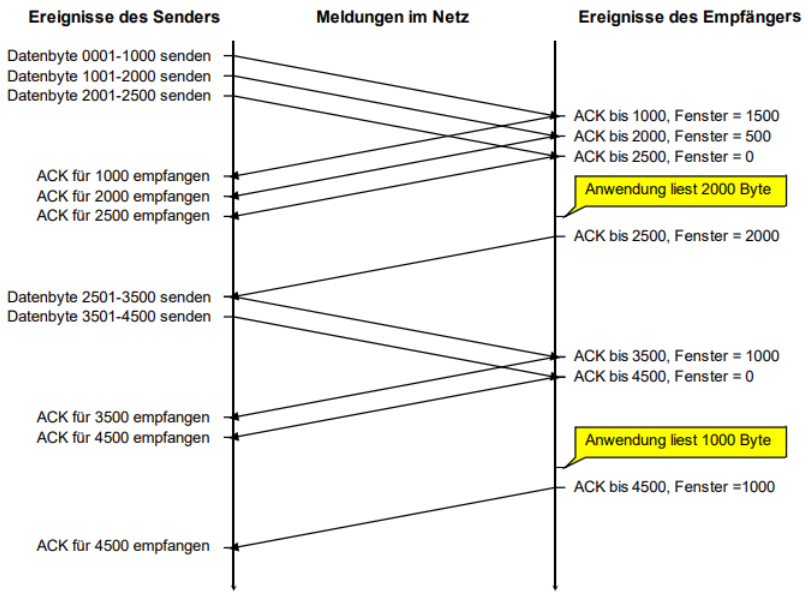
\includegraphics[width=1\linewidth]{images/flusssteuerung_tcp.png}\\
    Annahmen: 2'500 Byte Empfangspuffer, 5'000 Bytes Daten
    \begin{itemize}
        \item Fenstergrösse des Empfängers: WindowFeld des TCP-Headers
        \item Wireshark: Advertized Window Size
        \item Sender: nur einen Aufruf von send() für die gesamten 5'000 Bytes
    \end{itemize}
\end{example}



